\documentclass{standalone}
\usepackage{graphicx}
\begin{document}
\noindent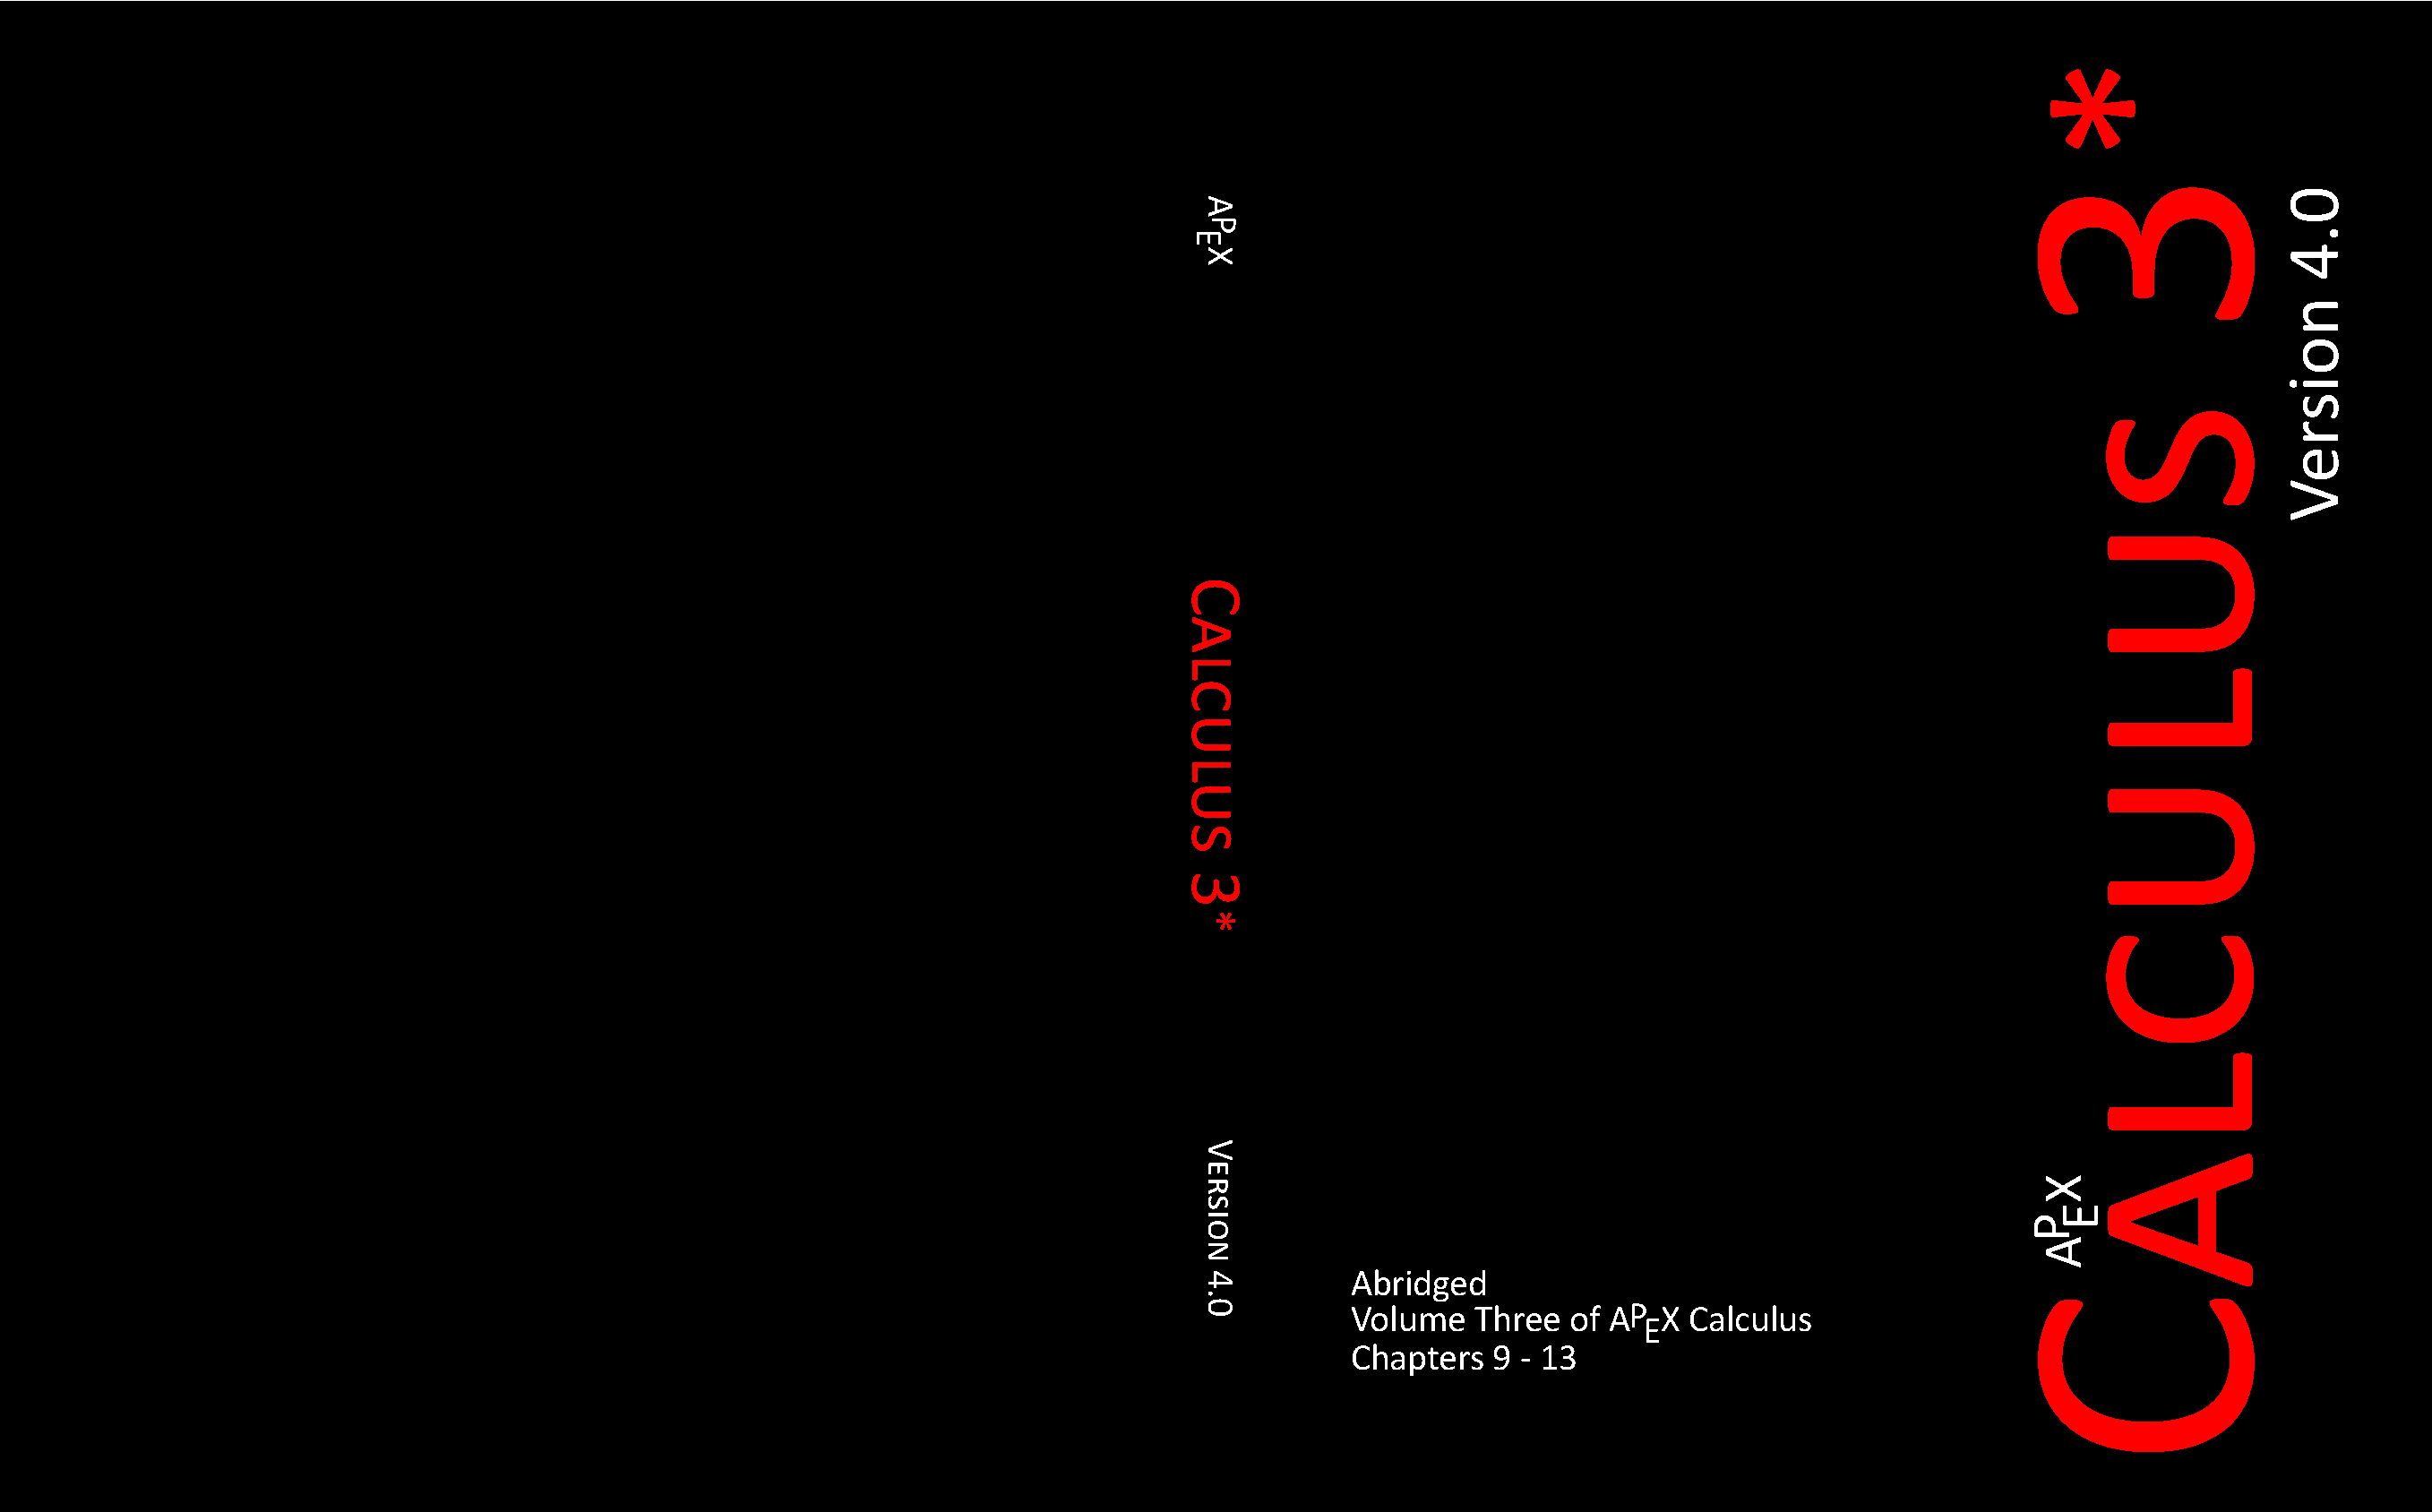
\includegraphics[height=2in,trim= 9.5in 0 0 0,clip]{amazon_createspace_cover_calculusIII_star}%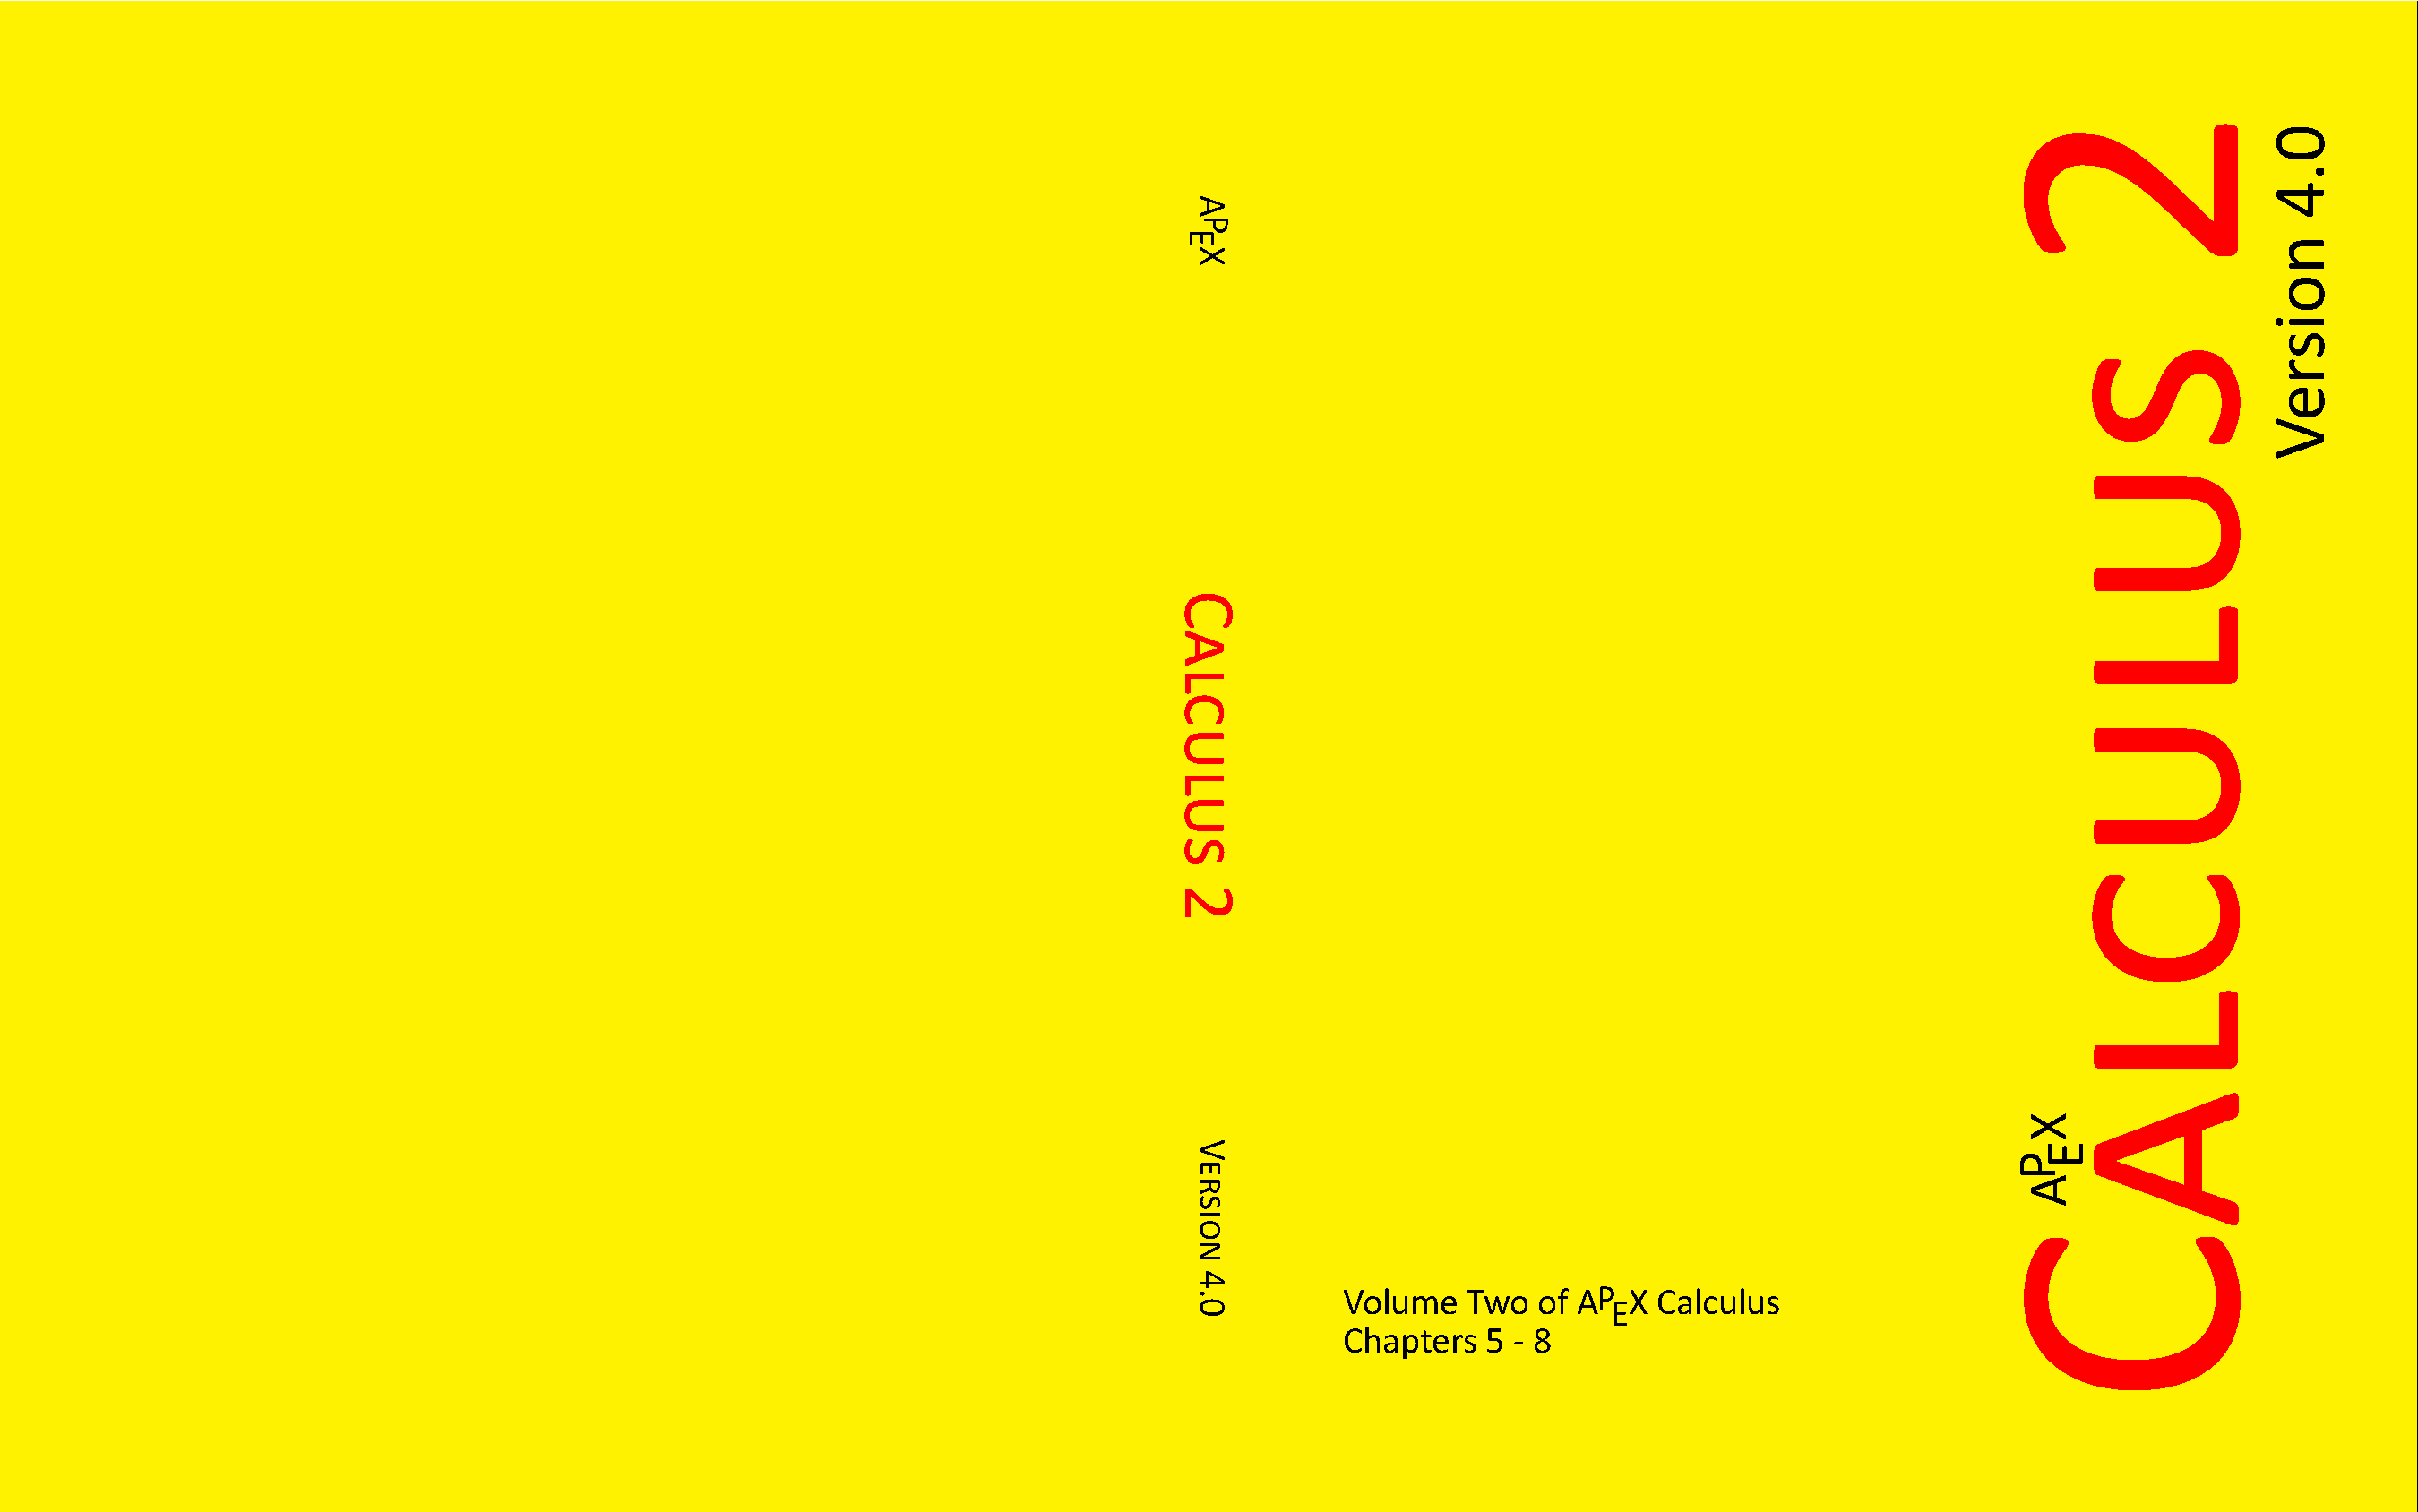
\includegraphics[height=2in,trim= 9.5in 0 0 0,clip]{amazon_createspace_cover_calculusII}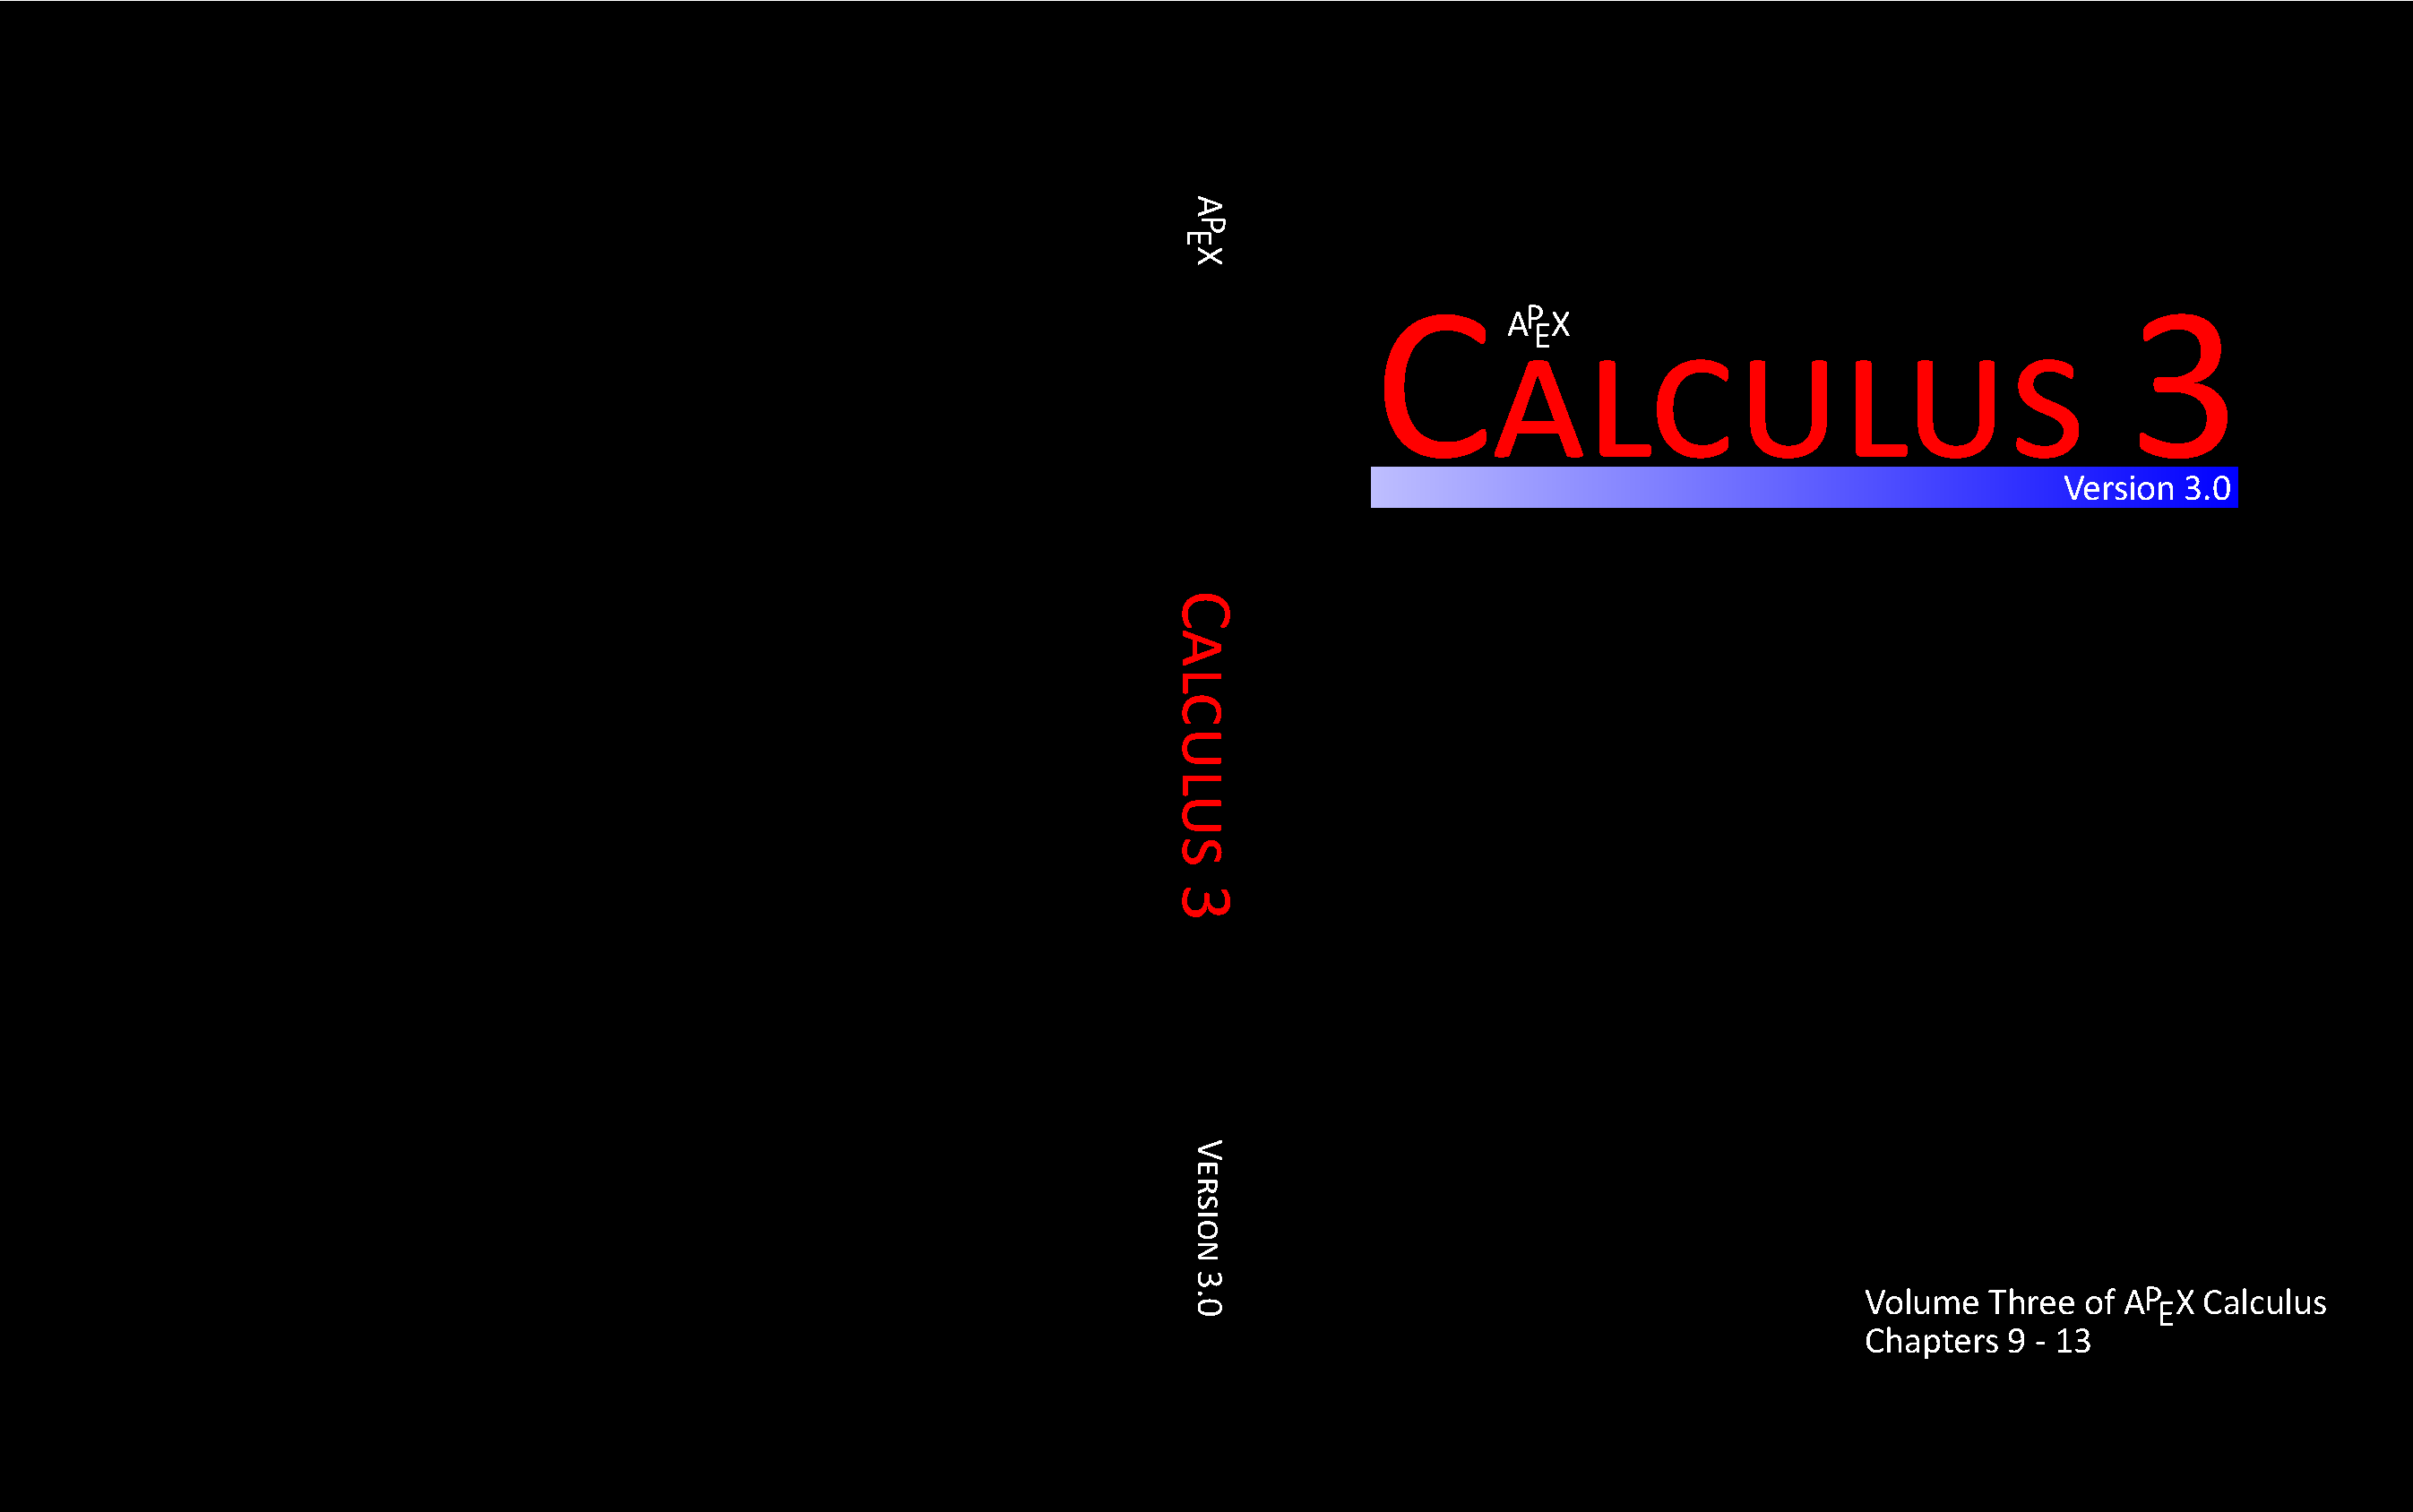
\includegraphics[height=2in,trim= 9.5in 0 0 0,clip]{amazon_createspace_cover_calculusIII}
\end{document}



%\documentclass{article}
%
%\usepackage{graphicx}
%\usepackage{tikz}
%\usepackage[paperwidth=17.95in,paperheight=11.25in]{geometry}
%
%\pagestyle{empty}
%
%\sffamily
	%%%\usepackage{fontspec}
	%\usepackage{mathspec}
	%\setallmainfonts[Mapping=tex-text]{Calibri}
	%\setmainfont[Mapping=tex-text]{Calibri}
	%\setsansfont[Mapping=tex-text]{Calibri}
	%\setmathsfont(Greek){[cmmi10]}
%
%
%
%\newcommand{\apex}{A\kern -1pt \lower -2pt\hbox{P}\kern -3pt \lower .65ex\hbox{E}\kern 0pt X}
%
%\begin{document}
%
%%\noindent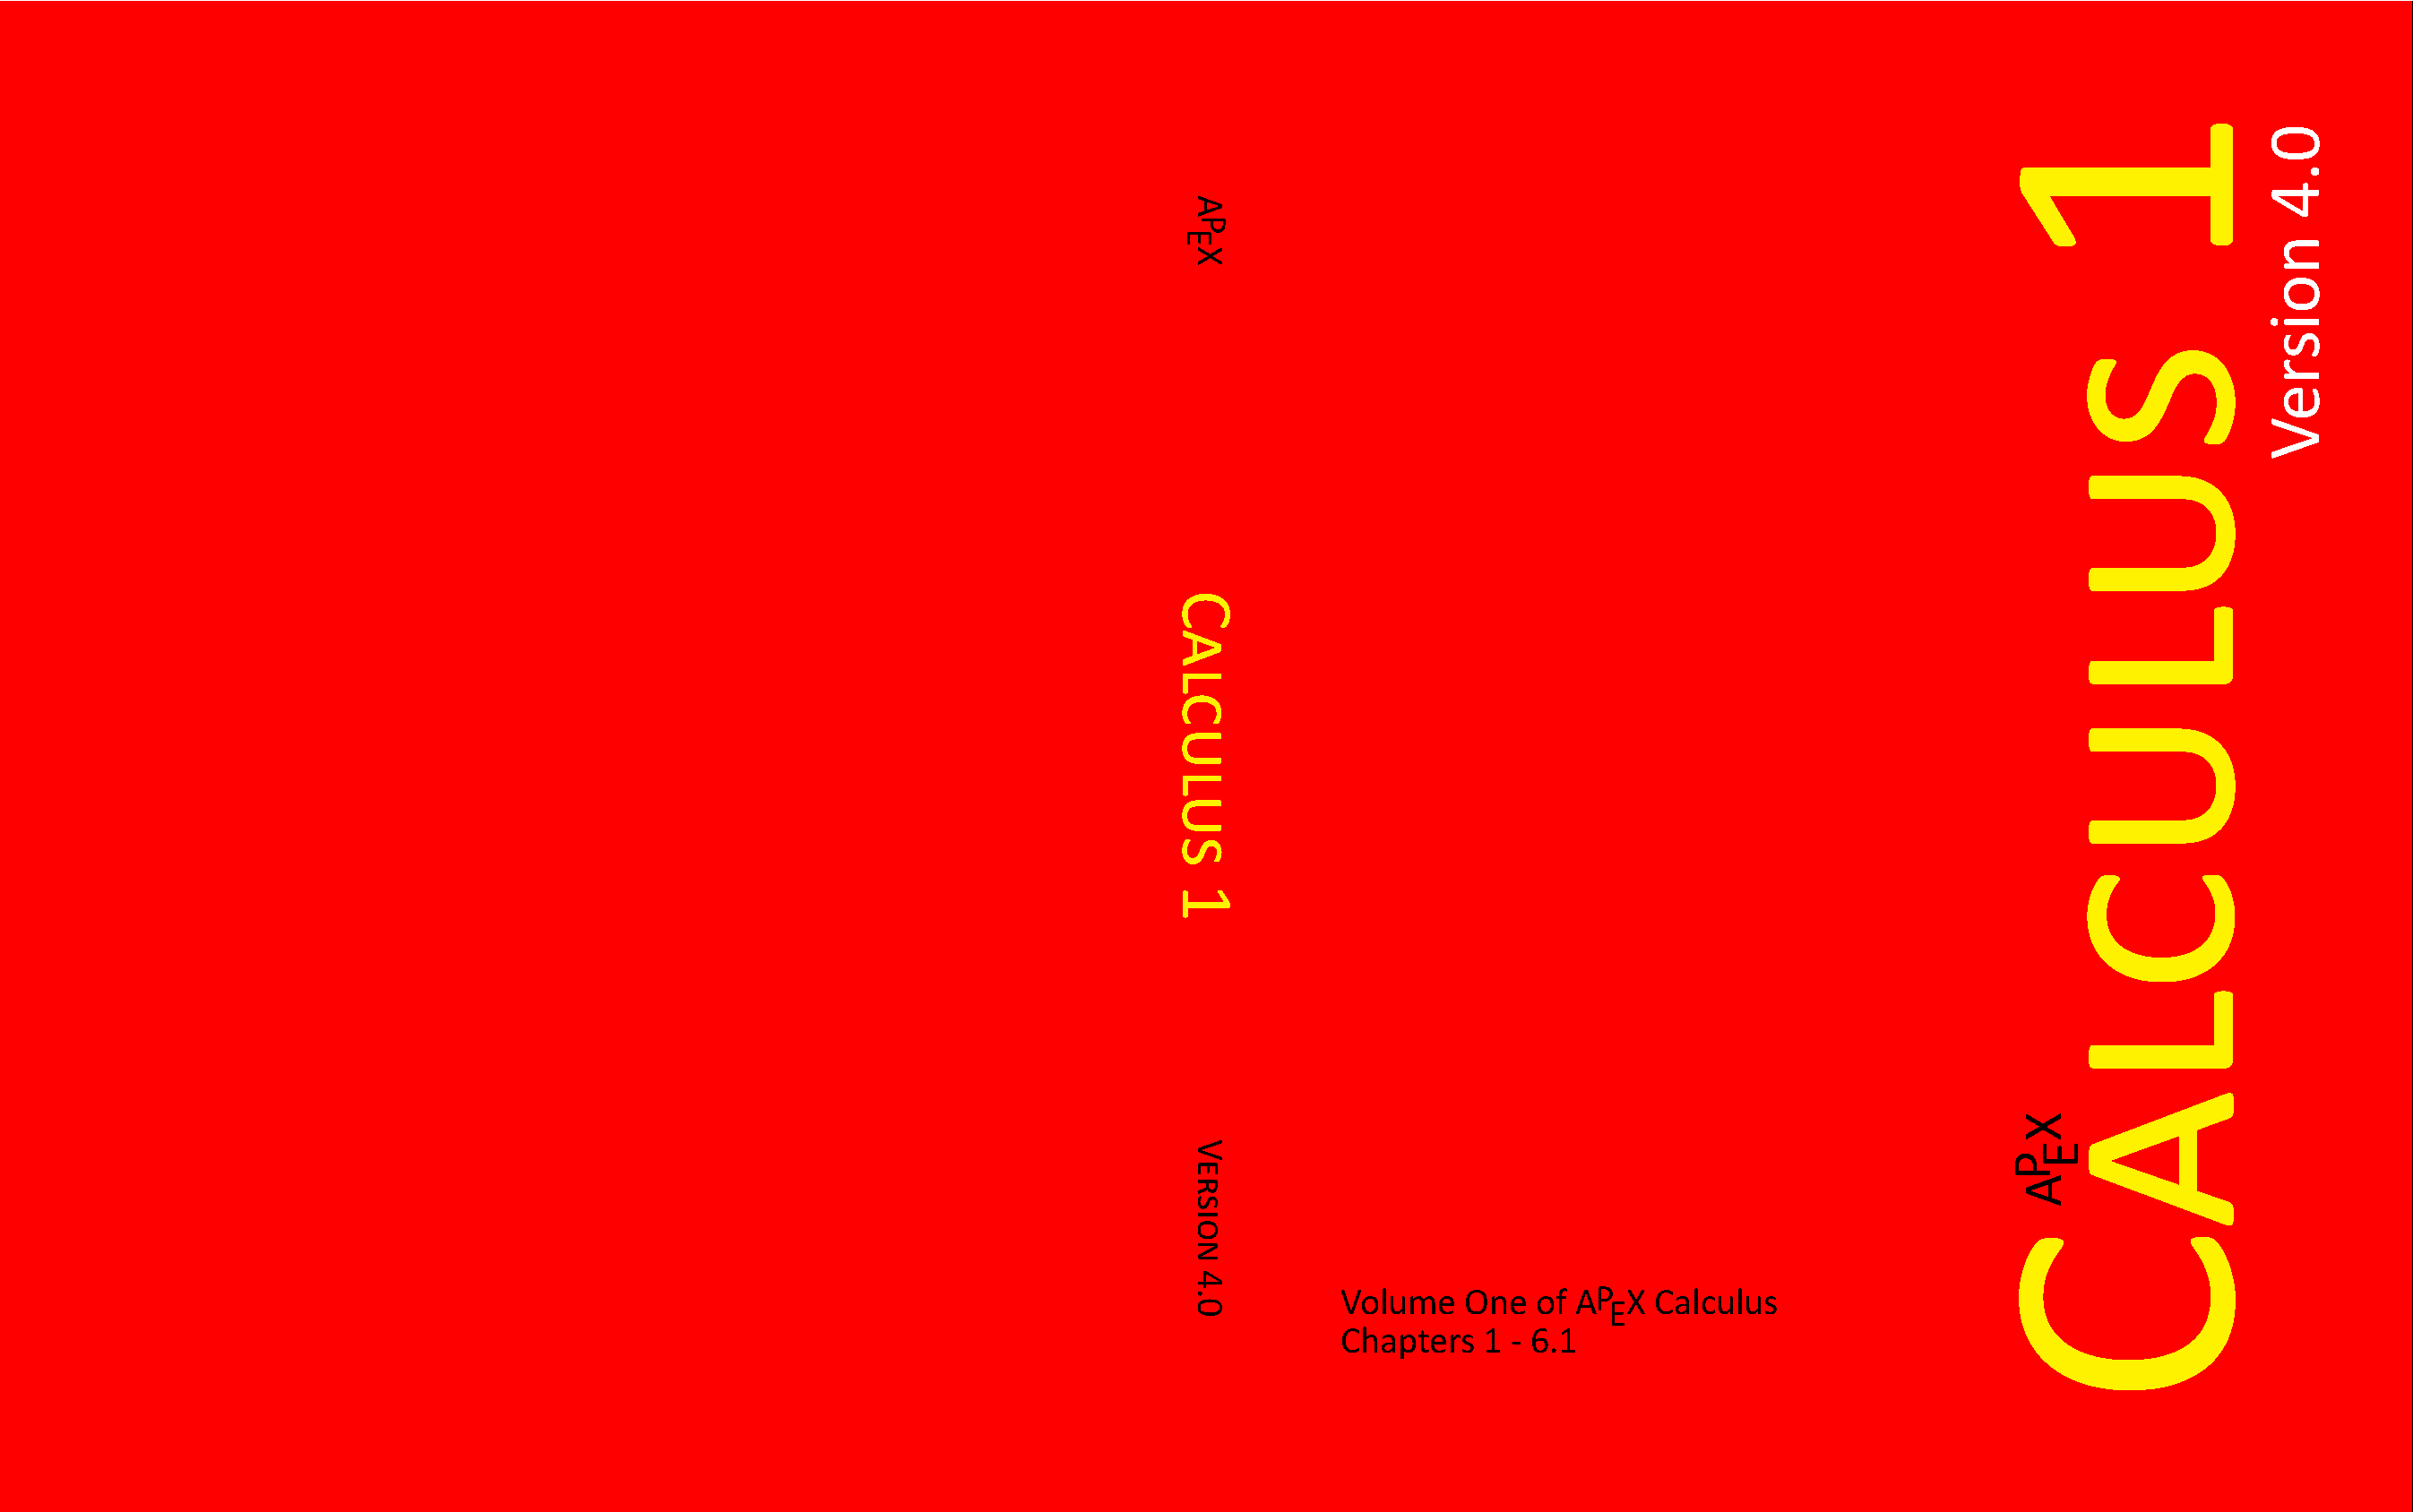
\includegraphics[height=2in,trim= 9.5in 0 0 0,clip]{amazon_createspace_cover_calculusI}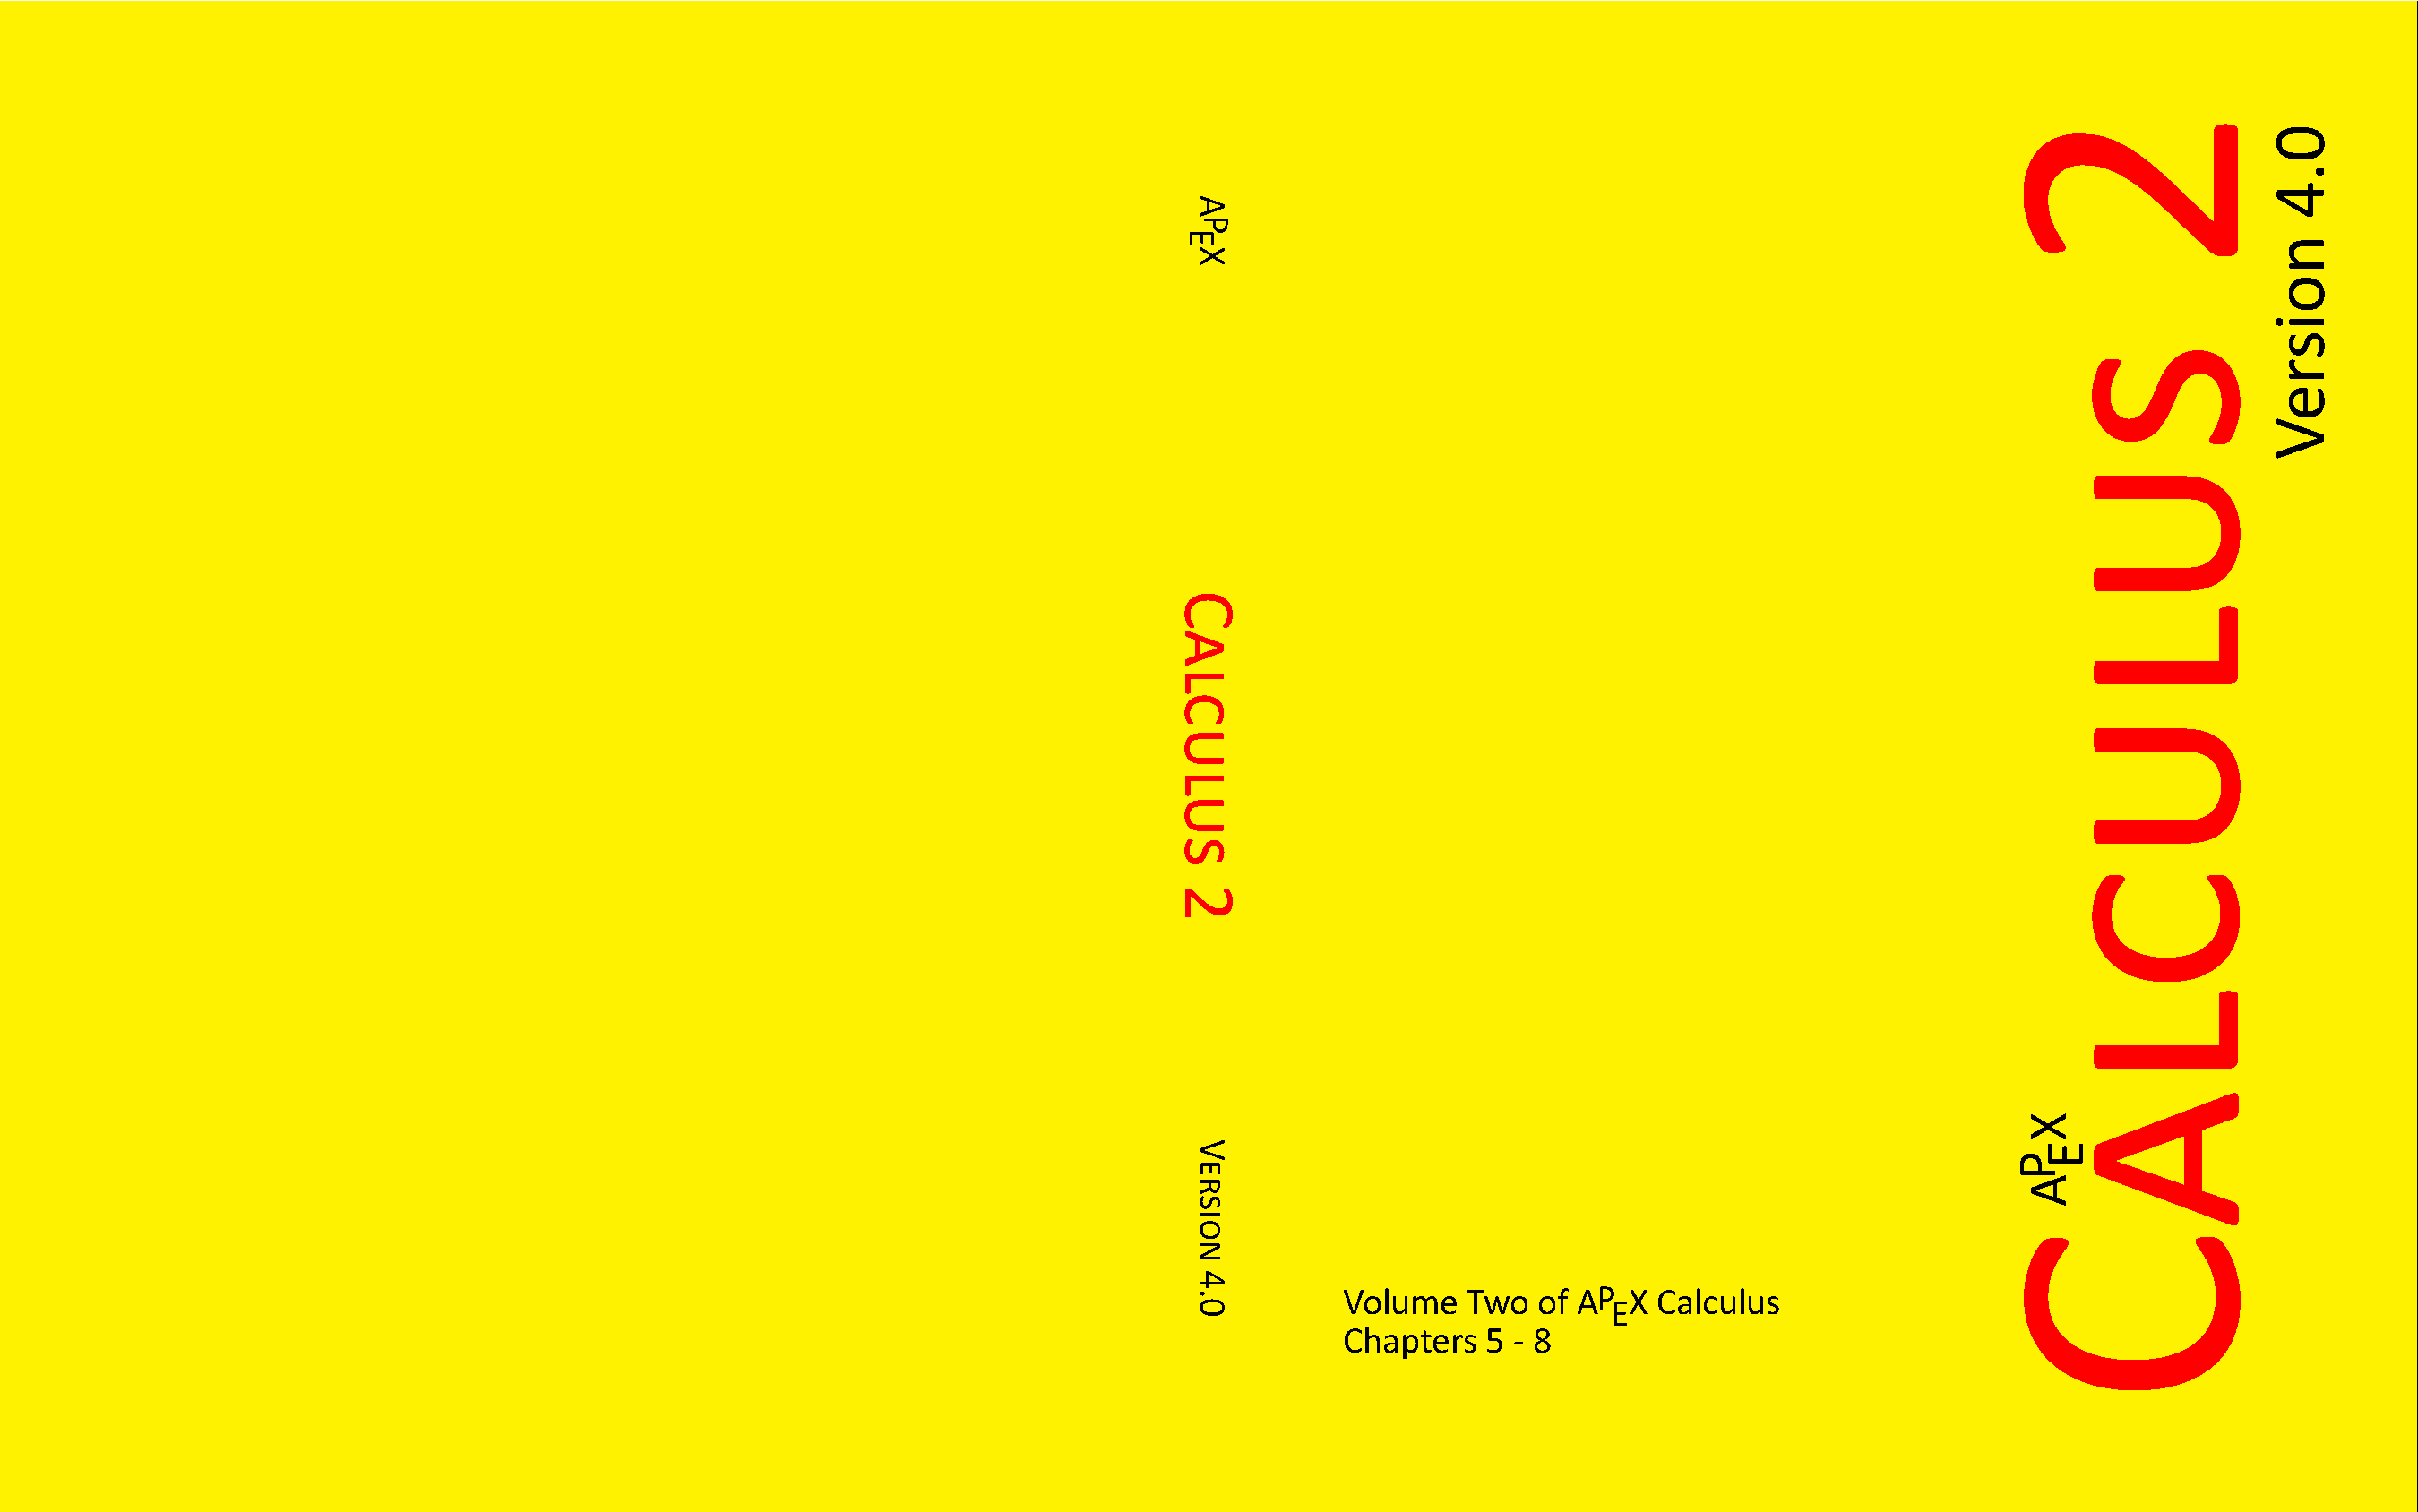
\includegraphics[height=2in,trim= 9.5in 0 0 0,clip]{amazon_createspace_cover_calculusII}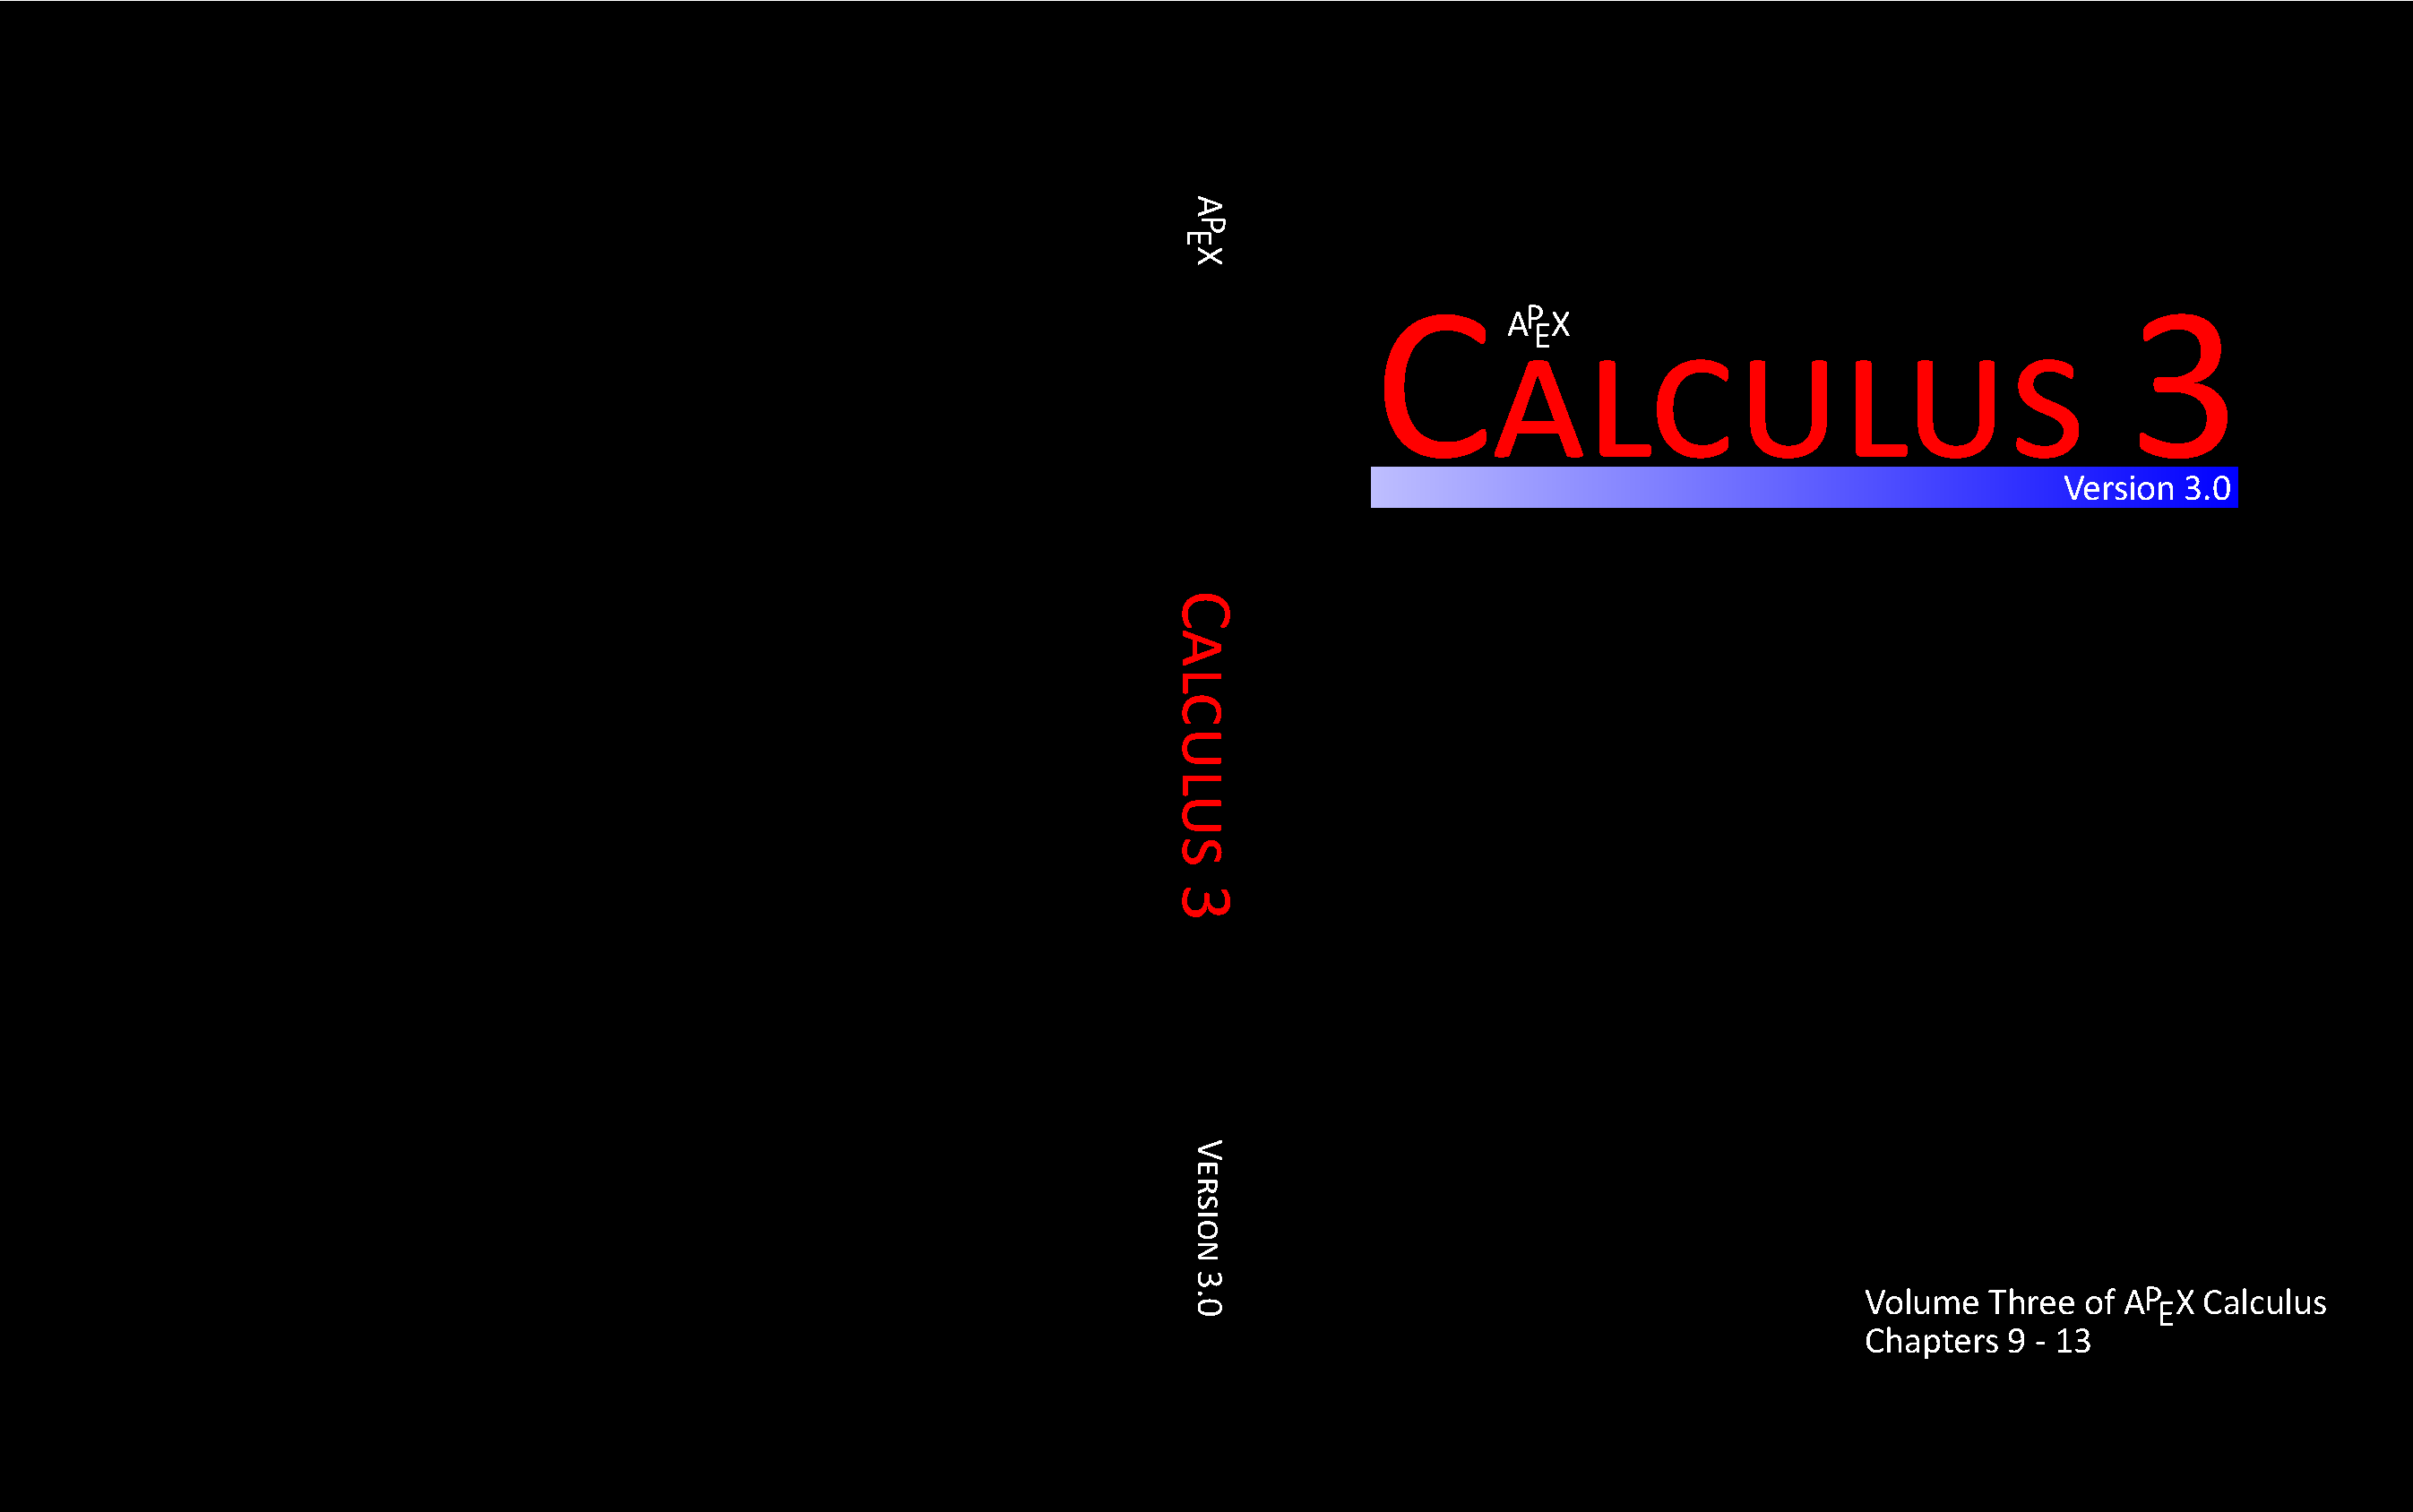
\includegraphics[height=2in,trim= 9.5in 0 0 0,clip]{amazon_createspace_cover_calculusIII}
%
%
%\begin{tikzpicture}%[remember picture,overlay]
%%\shade [bottom color=red!50!black,top color=red!70!black!60]
%%(top left) rectangle (bot right);
%%\draw [fill=red] (top left) rectangle (bot right);
%
%
%
%%%
%%% Draws lines for reference. Turn off for final product.
%%%%
%%\draw[green] (ptop left) -- (ptop right) -- (pbot right) -- (pbot left) -- (ptop left);
%%\draw [green] (lspine top) -- (lspine bot) (rspine top) -- (rspine bot);
%%\draw[green] (ptop right) -- (pbot left);
%
%\begin{scope}%[rotate=90]
%
%%\node[xshift=-.75in,yshift=0in,scale=4,white,right color=blue,left color=blue!25!white,transform shape,rotate=90] at ($.5*(ptop right)+.5*(pbot right)$) {\fontspec[Scale=1]{Calibri} \rule{0pt}{0pt} \parbox{170pt}{\hfill\ Version 4.0}\ };
%
%
%%\node [xshift=-2in,yshift=-3.in,black,scale=6,transform shape,rotate=90] at ($.5*(ptop right)+.5*(pbot right)$) {\fontspec[Scale=1]{Calibri} \apex};
%
%\node[xshift=0in,yshift=0in,scale=6,black] at (0,0) {\fontspec[Scale=3]{Calibri}\scshape C\fontspec[Scale=2.5]{Calibri}alculus};
%
%
%
%%\node[xshift=-.75in,yshift=3.5in,scale=4,white,transform shape,rotate=90] at ($.5*(ptop right)+.5*(pbot right)$) {\fontspec[Scale=1]{Calibri} Version 4.0};
%
%\node[xshift=0in,yshift=-1.25in,scale=4,red] at (0,0) {\fontspec[Scale=1]{Calibri} \parbox{140pt}{\hfill\ Version 4.0}};
%
%\node [xshift=-2.19in,yshift=0.6in,black,scale=3] at (0,0) {\fontspec[Scale=1]{Calibri} \apex};
%
%
%%\node[xshift=3.25in,yshift=3.2in,scale=3,black] at (current page.center) {\fontspec[Scale=1]{Calibri} \apex};
%
%\end{scope}
%\end{tikzpicture}
%
%\end{document}

